\documentclass[utf8,xcolor=table]{beamer}

\usepackage[T2A]{fontenc}
\usepackage[utf8]{inputenc}
\usepackage[english,russian]{babel}
\usepackage{minted}
\usepackage{ulem}
\usepackage{cmap}
\usepackage{multirow}

\hypersetup{colorlinks,linkcolor=blue,urlcolor=blue}

\mode<presentation>{
	\usetheme{CambridgeUS}
}

\renewcommand{\t}[1]{\ifmmode{\mathtt{#1}}\else{\texttt{#1}}\fi}
\newcommand{\svgimg}[1]{
  \begin{center}
	\includegraphics[width=\textwidth,height=0.8\textheight,keepaspectratio]{#1.pdf}
  \end{center}
}

\title[Многопоточность-1]{Многопоточность-1}
\author{Егор Суворов}
\institute[НИУ ВШЭ]{Курс <<Основы программирования>>}
\date[28.11.2019]{Четверг, 28 ноября 2019 года}

\setlength{\arrayrulewidth}{1pt}

\begin{document}

\begin{frame}
\titlepage
\end{frame}

\begin{frame}{План занятия}
	\tableofcontents
\end{frame}

\section{Параллельные вычисления}
\subsection{Зачем}

\begin{frame}
	\tableofcontents[currentsection,currentsubsection]
\end{frame}

\begin{frame}{Скорость вычислений}
	\begin{itemize}
		\item Хочется обрабатывать всё б\'{о}льшие объёмы информации всё быстрее.
		\item Пример: эмуляция движений воздуха на планете Земля за ближайшие 48 часов (прогноз погоды).
		\item Пока работает эмпирический \href{https://ru.wikipedia.org/wiki/\%D0\%97\%D0\%B0\%D0\%BA\%D0\%BE\%D0\%BD\_\%D0\%9C\%D1\%83\%D1\%80\%D0\%B0}{закон Мура}: каждые два года плотность транзисторов удваивается.
		\item Раньше это означало увеличение частоты процессора в два раза.
		\item Уже нет: процессор с частотой 2.8 ГГц был представлен в 2004 году (Pentium 4 Prescott).
		\item С тех пор скорость работы повышалась, но другими способами: размер кэша, скорость памяти, периферии...
		\item Уже уткнулись в ограничения размера процессора из-за скорости света.
	\end{itemize}
\end{frame}

\begin{frame}[fragile]{Параллелизм}
	\begin{itemize}
		\item Иногда можно работать быстрее, не увеличивая частоту, распараллелив команды:
\begin{minted}{cpp}
int x = a * b * 10;  // Нужен блок умножения.
int y = a / b;       // Нужен блок деления.
\end{minted}
		\item Процессоры умеют это автоматически детектировать без участия программистов.
		\item Компиляторы умеют передвигать операции так, чтобы процессору было проще.
		\item В последние годы активно появляются многоядерные процессоры: впихнуть второе ядро оказалось проще оптимизации физических процессов.
		\item Также можно использовать мощь б\'{о}льшего числа компьютеров (\href{https://ru.wikipedia.org/wiki/Folding@home}{Folding@Home}).
	\end{itemize}
\end{frame}

\begin{frame}{На домашнем компьютере}
	Идеи распараллеливания полезны и где-то, кроме ускорения:
	\begin{itemize}
		\item
			Обычные задачи дома не требуют большой вычислительной мощи:
			\begin{itemize}
				\item Процесс обычно ждёт реакции пользователя, диска или сети.
				\item Вычисления длятся не больше нескольких секунд.
			\end{itemize}
		\item Хочется свободно переключаться между приложениями и слушать музыку в фоне.
		\item Если есть ресурсоёмкая задача, нестрашно, если она будет выполняться чуть медленнее.
		\item На телефоне одно ядро может целиком отрисовывать нетормозящий интерфейс, а другое "--- производить вычисления.
		\item Пример: AlarmUserHandler из предыдущего домашнего задания.
	\end{itemize}
\end{frame}

\subsection{Как}
\begin{frame}[fragile]{Параллельные алгоритмы}
	\begin{itemize}
		\item Некоторые алгоритмы параллелятся просто:
\begin{minted}{cpp}
int sum = 0;
for (int x : values) sum += x;
\end{minted}
		\item Некоторые "--- естественно и на уровне железа:
\begin{minted}{cpp}
char buf1[100], buf2[100];
fread(file_on_disk1, 1, sizeof buf1, buf1);
fread(file_on_disk2, 1, sizeof buf2, buf2);
\end{minted}
		\item Некоторые не параллелятся:
\begin{minted}{cpp}
int steps = 0;
for (int x = 1; x != 0; x = f(x)); steps++;
\end{minted}
		\item Надо писать специальные алгоритмы для распределённых вычислений.
		\item Иногда перебор параллелится лучше умного решения.
	\end{itemize}
\end{frame}

\begin{frame}{Иллюстрация}
	\begin{center}
		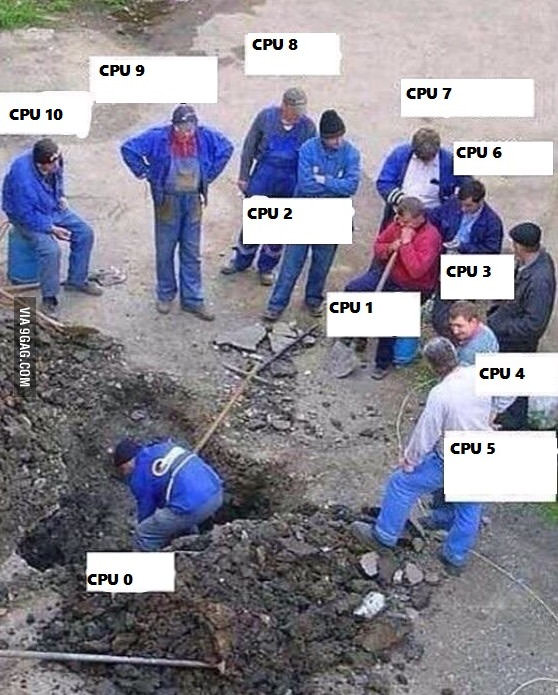
\includegraphics[height=6cm]{cpus-joke.jpg}

		Простое добавление ядер не увеличивает производительность!
	\end{center}
\end{frame}

\begin{frame}{В прикладном хозяйстве}
	\begin{itemize}
		\item Современные ОС различают \textit{потоки} и \textit{процессы}.
		\item Процесс "--- это обычно одно приложение (браузер, IDE, веб-сервер...), у которого может быть много потоков.
		\item Например: у браузера один поток на вкладку; у веб-сервера "--- один поток на клиента.
		\item Изначально у процесса есть только один поток (\textit{главный}), он может создавать другие.
		\item Более строго: процесс "--- это некоторое множество потоков, у которых общая память и другие ресурсы (открытые файлы).
		\item Поток "--- это что-то, выполняющее некий код (есть отдельный стек, свои данные в регистрах процессора, свой код).\
	\end{itemize}
\end{frame}

\begin{frame}{С точки зрения программиста}
	\begin{itemize}
		\item На разных ОС разные методы для работы с процессами или потоками.
		\item Напрямую API уровня ОС, как обычно, никто не использует.
		\item В языках высокого уровня (Java, Python) обычно есть соответствующая библиотека.
		\item Также есть другие классические библиотеки и стандарты:
			\begin{itemize}
				\item pthread "--- Posix Thread, стандарт в C. Будем использовать.
				\item OpenMP "--- высокоуровневое распараллеливание для C/C++/Fortran.
				\item CUDA "--- вычисления на графических картах (ядер тысячи, но они умеют меньше, чем CPU).
			\end{itemize}
	\end{itemize}
\end{frame}

\begin{frame}[fragile]{Типичный псевдокод-1}
\begin{minted}{cpp}
void draw() {
    while (true) {
        wait_for_events();
        process_updates();
        process_mouse_events();
        repaint();
    }
}
int main() {
    Thread draw_thread(draw);
    draw_thread.start();
    // ...
    add_rectangle(10, 10, 30, 40);
    // ...
}
\end{minted}
\end{frame}

\begin{frame}[fragile]{Типичный псевдокод-2}
\begin{minted}{cpp}
void process_client(Client client) {
    string request = client.read();
    string answer = "I've got " + request;
    client.write(answer);
}
int main() {
    while (true) {
        Client client = get_next_client();
        Thread(process_client, client).start();
    }
}
\end{minted}
\end{frame}

\begin{frame}{Producer-Consumer}
	\svgimg{prod-cons}
\end{frame}

\begin{frame}[fragile]{Типичный псевдокод-3}
\begin{minted}{cpp}
void merge_sort(int l, int r) {
    if (l + 1 == r) return;
    Thread t1(merge_sort, l, (l + r) / 2);
    Thread t2(merge_sort, (l + r) / 2, r);
    t1.start(); t2.start(); // Запускаем потоки.
    t1.join(); t2.join();   // Ждём завершения.
    merge(l, r);
}
\end{minted}
\end{frame}

\section{Практические грабли}
\subsection{Простое приложение на pthread}

\begin{frame}
	\tableofcontents[currentsection,currentsubsection]
\end{frame}

\begin{frame}{Что такое pthread}
	\begin{itemize}
		\item Стандартный интерфейс функций для работы с потоками (POSIX Threads).
		\item Есть реализации под Windows, Linux и другие ОС.
		\item Стандарт при разработке программ на C.
		\item Имена функций и типов начинаются с \t{pthread\_}.
		\item В Linux можно получить справку, набрав \t{man <имя функции>} в консоли.
		\item Под остальными "--- то же самое, но в гугле.
	\end{itemize}
\end{frame}

\begin{frame}[fragile]{Один поток}
	\svgimg{simple-one-thread}
\end{frame}

\begin{frame}[fragile]{Много потоков}
	\svgimg{simple-two-threads}
\end{frame}

\begin{frame}[fragile]{Пример кода}
	Демо \texttt{01-simple.cpp}
\end{frame}

\begin{frame}{Как живут потоки}
	\begin{itemize}
		\item При создании потока при помощи \t{pthread\_create} указывается функция и её аргумент "--- один указатель на что угодно.
		\item Вернуть функция тоже может указатель на что угодно.
		\item Поток завершается, когда функция делает \t{return} или \t{pthread\_exit}.
		\item Указатель на поток хранится в переменной типа \t{pthread\_t}.
		\item При создании потока он сразу начинает выполняться.
		\item \t{pthread\_join} делает следующее:
			\begin{enumerate}
				\item Ждёт окончания работы потока.
				\item Освобождает все ресурсы потока (стек).
				\item Возвращает то, что вернула функция потока.
			\end{enumerate}
		\item Когда \t{main} делает \t{return 0} или вы вызываете \t{exit(0)}, умирает весь процесс со всеми потоками.
		\item Но в \t{main} можно сделать \t{pthread\_exit}, если очень хочется, тогда процесс не умрёт, пока живы потоки.
	\end{itemize}
\end{frame}

\begin{frame}{Демо detached}
	Демо \texttt{02-detached.cpp}
	% data стала глобальной, arg не нужен
	% pthread_detach (падает)
	% убираем pthread_join (не всегда успевает отработать)
	% pthread_exit в main (теперь окей)
\end{frame}

\begin{frame}[t]{Несколько замечаний про pthread}
	Про потоки и pthread:
	\begin{itemize}
		\item Использовать \t{void* arg} и возвращаемое значение для передачи данных необязательно.
		\item Вся память внутри процесса одинаково доступна всем потокам на чтение и запись.
		\item \t{void* arg} возникает только тогда, когда надо запустить потоки на разных данных.
		\item
			Что произойдёт, если мы забудем \t{join} и \t{main} завершится до начала \t{worker}?
			Предполагаем, что процесс при этом не умрёт.
			\only<2->{Неопределённое поведение "--- \t{worker} попытается изменить переменную \t{data}, которая уже исчезла.}
	\end{itemize}
\end{frame}

\begin{frame}{Кто освобождает ресурсы?}
	На самом деле в pthread есть два типа потоков: joinable и detached.

	Joinable:
	\begin{itemize}
		\item Тип по умолчанию.
		\item На таком потоке должен быть ровно один раз вызыван метод \t{pthread\_join}, который освободит ресурсы и сообщит, что поток вернул.
		\item Если не вызвать "--- ресурсы не будут освобождены до конца программы.
		\item Если вызвать дважды "--- второй вызов может уронить программу или вернуть неверный результат.
	\end{itemize}

	Detached:
	\begin{itemize}
		\item Система автоматически освободит ресурсы как только поток завершится.
		\item Нельзя вызывать \t{pthread\_join} и получать возвращаемое значение "--- его негде хранить после окончания работы.
	\end{itemize}
\end{frame}

\begin{frame}{В других системах}
	\begin{itemize}
		\item Joinable/detached также используется в Java.
		\item В Windows (не в pthread под Windows!) другая концепция:
			\begin{itemize}
				\item Указатель на поток "--- сложный объект, который надо запрашивать у ОС и освобождать (как \t{FILE*}), а не просто переменная.
				\item Ресурсы потока освобождаются, когда он завершился и на него больше нет указателей.
				\item Нет разделения joinable/detached.
				\item Если кто-то может спросить состояние потока "--- у него есть указатель, значит, ресурсы потока ещё не освобождены.
			\end{itemize}
	\end{itemize}
\end{frame}

\subsection{Состояние гонки}

\begin{frame}
	\tableofcontents[currentsection,currentsubsection]
\end{frame}

\begin{frame}{Демо гонки-1}
	Демо: \texttt{03-writeln-single}, \texttt{04-writeln-single}

	Valgrind не помогает.
\end{frame}

\begin{frame}{Объяснение}
	\begin{itemize}
		\item
			Потоки выполняют команды <<одновременно>>.
			Если есть доступ к общему ресурсу (экран), то порядок не определить.
		\item
			Поэтому символы выводятся вперемешку.
		\item
			\textit{Состояние гонки} (\textit{race condition}) "--- это когда результат работы зависит от того, в каком порядке потоки выполняли команды.
		\item
			Самая популярная ошибка у начинающих.
		\item
			Операция называется \textit{атомарной}, если она всегда выполняется <<за один такт>>,
			то есть другие потоки не видят её частично выполненной.
		\item
			\t{writeln} выше не атомарна.
	\end{itemize}
\end{frame}

\begin{frame}{Состояние гонки: повезло}
	\svgimg{race-writeln-ok}
\end{frame}

\begin{frame}{Состояние гонки: не повезло}
	\svgimg{race-writeln-bad}
\end{frame}

\begin{frame}{Демо гонки-2}
	Демо: \texttt{05-counter.cpp}, \texttt{06-even-counter.cpp}

	Важно: оптимизации отключены! (почему "--- на следующей лекции).

	Valgrind не помогает.
\end{frame}

\begin{frame}{Объяснение}
	Возможная последовательность действий:
	\begin{itemize}
		\item Основной поток: \t{if (data \% 2 == 0)} $\to \t{true}$.
		\item Второй поток: \t{data++}.
		\item Основной поток: \t{printf}.
	\end{itemize}
	Как исправить?
	\pause
	\begin{itemize}
		\item Можно на каждой итерации записать значение \t{data} в локальную \t{data\_snapshot} (снимок) и работать с ним.
		\item Работает только если чтение одной переменной атомарно.
		\item Не работает, если у нас много переменных мы не можем сделать атомарный снимок (классическая задача).
		\item Демо: \texttt{07-even-counter-snapshot.cpp}
	\end{itemize}
\end{frame}

\begin{frame}{Иллюстрация}
	\begin{center}
		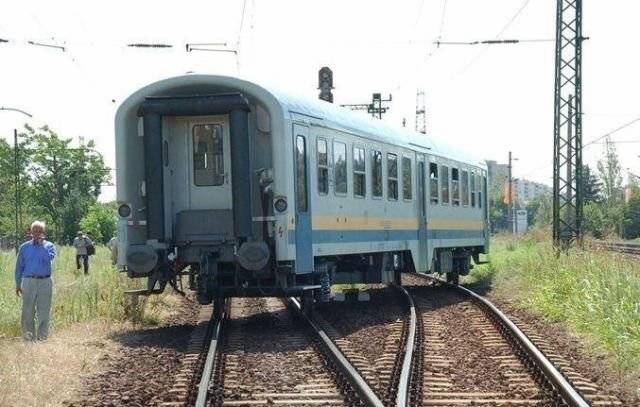
\includegraphics[scale=0.6]{race-condition.jpg}
	\end{center}
\end{frame}

\subsection{Гонка данных}
\begin{frame}{Демо гонки-3}
	Демо: \texttt{08-two-threads.cpp}

	Valgrind, внезапно, помогает (как и thread sanitizer).
\end{frame}

\begin{frame}[fragile]{Состояние гонки: повезло}
	\svgimg{race-two-inc-good}
\end{frame}

\begin{frame}[fragile]{Состояние гонки: не повезло}
	\svgimg{race-two-inc-bad}
\end{frame}

\begin{frame}{А что вообще атомарно?}
	\begin{center}
		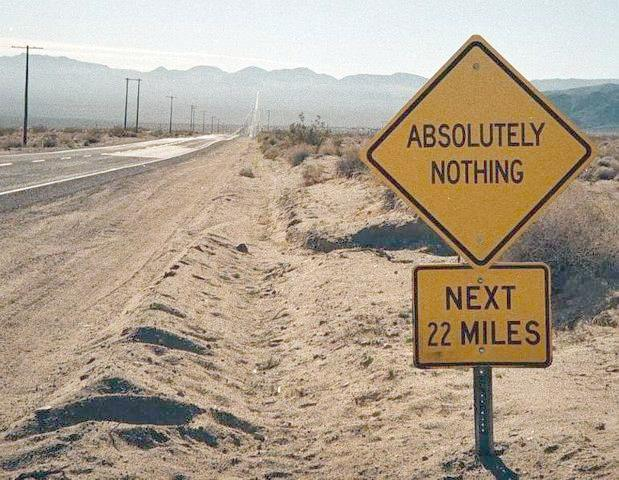
\includegraphics[scale=0.4]{absolutely-nothing.jpg}
	\end{center}

	Даже в Python или Java.
\end{frame}

\begin{frame}{Полезные советы}
	\begin{itemize}
		\item
			Что атомарно "--- очень сильно зависит от платформы, языка и ключей компиляции
			(<<модель памяти>>).
		\item Не пытайтесь угадать.
		\item Не пытайтесь самостоятельно писать код, зависящий от атомарности.
		\item В некоторых языках бывает \t{AtomicInteger} и похожие структуры.
		\item За ними тоже надо аккуратно следить, обычно не используют.
		\item Мораль из Rust:
			\begin{itemize}
			\item Несколько потоков, читающих одну переменную "--- окей
			\item Если кто-то пишет в переменную, то никто другой не может её читать
			\end{itemize}
	\end{itemize}
\end{frame}

\subsection{Взаимное исключение}

\begin{frame}
	\tableofcontents[currentsection,currentsubsection]
\end{frame}

\begin{frame}{Как избежать гонок}
	\begin{itemize}
		\item Можно обозначить кусок кода как \textit{критическую секцию} (critical section).
		\item Каждую критическую секцию может выполнять максимум один поток.
		\item
			Если весь доступ к общим данным обозначить как критическую секцию,
			то он станет де-факто атомарным.
		\item С каждой критической секцией ассоцириуется \textit{блокировка} (lock).
		\item При входе в секцию блокировку надо \textit{взять}/\textit{захватить} (acquire).
		\item При выходе из секции блокировку надо \textit{отпустить} (unlock/release).
		\item Другие названия блокировок: монитор (monitor), мьютекс (mutex, \textbf{mut}al \textbf{ex}clusion).
		\item Обычно реализованы на уровне ОС и все операции с ними медленные.
	\end{itemize}
\end{frame}

\begin{frame}{Мьютекс}
	\svgimg{mutex-good}
\end{frame}

\begin{frame}[fragile]{Некорректный пример}
\begin{minted}{cpp}
int data;
void* worker(void*) {
    pthread_mutex_t m;
    pthread_mutex_init(&m, NULL);
    for (int i = 0; i < N; i++) {
        pthread_mutex_lock(&m);
        data++;
        pthread_mutex_unlock(&m);
    }
    pthread_mutex_destroy(&m);
    return NULL;
}
\end{minted}
\href{https://raw.githubusercontent.com/yeputons/spring-2019-paradigms/master/190410/sources/09-two-threads-bad-mutex.cpp}{Код}.
\end{frame}

\begin{frame}[fragile]{Корректный пример}
\begin{minted}{cpp}
int data;
pthread_mutex_t m;
void* worker(void*) {
    for (int i = 0; i < N; i++) {
        pthread_mutex_lock(&m);
        data++;
        pthread_mutex_unlock(&m);
    }
    return NULL;
}
// ...
  pthread_mutex_init(&m, NULL);
// ...
  pthread_mutex_destroy(&m);
// ...
\end{minted}
\end{frame}

\begin{frame}{Упражнение}
	\begin{enumerate}
		\item Добавьте мьютекс в \href{https://raw.githubusercontent.com/yeputons/spring-2019-paradigms/master/190410/sources/08-two-threads.cpp}{двойной счётчик}.
		\item Уменьшите $N$ на несколько порядков (мьютексы сильно замедляют программу).
		\item Убедитесь, что всегда выводится $2N$.
		\item Добавьте мьютекс в \href{https://raw.githubusercontent.com/yeputons/spring-2019-paradigms/master/190410/sources/04-writeln-race.cpp}{writeln}.
	\end{enumerate}
	\href{https://raw.githubusercontent.com/yeputons/spring-2019-paradigms/master/190410/sources/10-two-threads-good-mutex.cpp}{Исправленный двойной счётчик},
	\href{https://raw.githubusercontent.com/yeputons/spring-2019-paradigms/master/190410/sources/11-writeln-mutex.cpp}{исправленный writeln}.
\end{frame}

\begin{frame}[fragile]{Блокировка}
	\begin{itemize}
		\item \t{pthread\_mutex\_lock} блокируется и ждёт, пока блокировка не станет доступна для захвата.
		\item Есть ли проблемы в следующем псевдокоде?
\begin{minted}{cpp}
void thread1() {
    m1.lock(); m2.lock();
    // ...
    m2.unlock(); m1.unlock();
}
void thread2() {
    m2.lock(); m1.lock();
    // ...
    m1.unlock(); m2.unlock();
}
\end{minted}
	\end{itemize}
\end{frame}

\begin{frame}{Взаимная блокировка}
	\begin{center}
		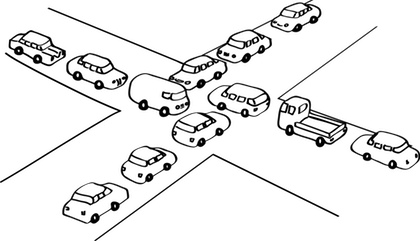
\includegraphics{deadlock.jpg}
	\end{center}
	\begin{itemize}
		\item
			Может случиться проблема:
			\begin{enumerate}
				\item Поток 1 захватывает \t{m1}.
				\item Поток 2 захватывает \t{m2}.
				\item Поток 1 не может захватить \t{m2}.
				\item Поток 2 не может захватить \t{m1}.
				\item Оба потока встали в \textit{deadlock} (\textit{взаимная блокировка}).
			\end{enumerate}
		\item
			Решение: всегда брать блокировки в одном и том же порядке.
			Тогда можно доказать, что deadlock такого вида не образуется.
		\item
			Если ввести линейный порядок на мьютексах не получается, у вас проблема.
	\end{itemize}
\end{frame}

\begin{frame}[fragile]{Мьютексы "--- не панацея}
\begin{minted}{cpp}
void inc() {  // Атомарна.
    m.lock(); data++; m.unlock();
}
void double_inc() {  // Не атомарно.
    inc(); inc();
}
void check() {
    m.lock();
    assert(data % 2 == 0);
    m.unlock();
}
\end{minted}
	\begin{itemize}
		\item Код выше может упасть, даже если вызывать только \t{double\_inc}.
		\item Мьютекс в простом случае лишь добавляет атомарности.
		\item Две атомарные операции подряд, как и раньше, атомарную вместе не образуют.
	\end{itemize}
\end{frame}

\begin{frame}[fragile]{Reentrant}
\begin{minted}{cpp}
void inc() {  // Атомарна.
    m.lock(); data++; m.unlock();
}
void double_inc() {  // Атомарно?
    m.lock(); inc(); inc(); m.unlock();
}
\end{minted}
	\begin{itemize}
		\item \t{double\_inc} заблокируется, так как \t{inc} попробует взять мьютекс второй раз.
		\item Есть специальный вид мьютексов, которые позволяют захватывать себя ещё раз из того же потока, называется \textit{reentrant}.
		\item Их обычно не используют "--- они сложнее в реализации.
	\end{itemize}
\end{frame}

\begin{frame}[fragile]{Решение}
	Вынести специальную функцию для внутреннего использования, которая предполагает, что блокировка уже взята:
\begin{minted}{cpp}
void inc_lock_held() { data++; }  // Приватная
void inc() {
    m.lock(); inc_lock_held(); m.unlock();
}
void double_inc() {
    m.lock();
    inc_lock_held(); inc_lock_held();
    m.unlock();
}
\end{minted}
	В ООП функция \t{inc\_lock\_held} обязательно была бы приватной.
\end{frame}

\begin{frame}[fragile]{Блокировка "--- ресурс}
	Есть ли проблема?
\begin{minted}{cpp}
void inc_special() {
    m.lock();
    if (condition()) return;
    data++;
    m.unlock();
}
\end{minted}
	\pause
	\begin{itemize}
		\item Есть: блокировка может быть не отпущена в случае досрочного \t{return}.
		\item Тогда \t{m} больше никто никогда не захватит и все следующие вызовы \t{inc\_special} не смогут начаться.
		\item Вам поможет привычка всегда освобождать взятые ресурсы (файлы, память, \textit{мьютекс}).
		\item Или специальный синтаксический сахар вроде RAII в C++, или try-with-resources/synchronized-блоков в Java.
	\end{itemize}
\end{frame}

\begin{frame}[fragile]{Синтаксический сахар}
	Идиома \textit{RAII}:
\begin{minted}{cpp}
void inc_special() {
    ScopedLock lock(m);  // Берём блокировку в конструкторе
    if (condition()) return;
    data++;
}  // Освобождаем в деструкторе.
\end{minted}

	synchronized-блоки в Java (каждый получит мьютекс):
\begin{minted}{java}
void inc_special() {
    synchronized {
        if (condition()) return;
        data++;
    }
}
\end{minted}
\end{frame}

\begin{frame}{Резюме}
	\begin{itemize}
		\item Атомарные операции в потоках могут выполняться в любом порядке, если их не синхронизировать.
		\item Вы обычно не знаете, что атомарно, а что нет.
		\item \textit{Любой} доступ к общим ресурсам должен быть \textit{защищён} (guarded) блокировкой.
		\item В частности, любая переменная, доступная из нескольких потоков, должна быть защищена \textit{ровно} одной блокировкой (почему?).
		\item Блокировки надо брать всегда в одном и том же порядке.
		\item Если пишете потокобезопасный объект, блокировку надо брать на самой <<верхней>> операции, которая должна быть атомарной.
		\item Дубовый способ переделки \textit{потоконебезопасной} структуры в безопасную: создать один мьютекс и брать его на каждую операцию со структурой.
		\item Мьютексы сильно тормозят, лучше вообще избегать общего доступа к данным (и меньше шанс набагать), привет из Rust.
	\end{itemize}
\end{frame}

\section{Отладка}

\begin{frame}
	\tableofcontents[currentsection,currentsubsection]
\end{frame}

\begin{frame}{Как отлаживать}
	\begin{center}
		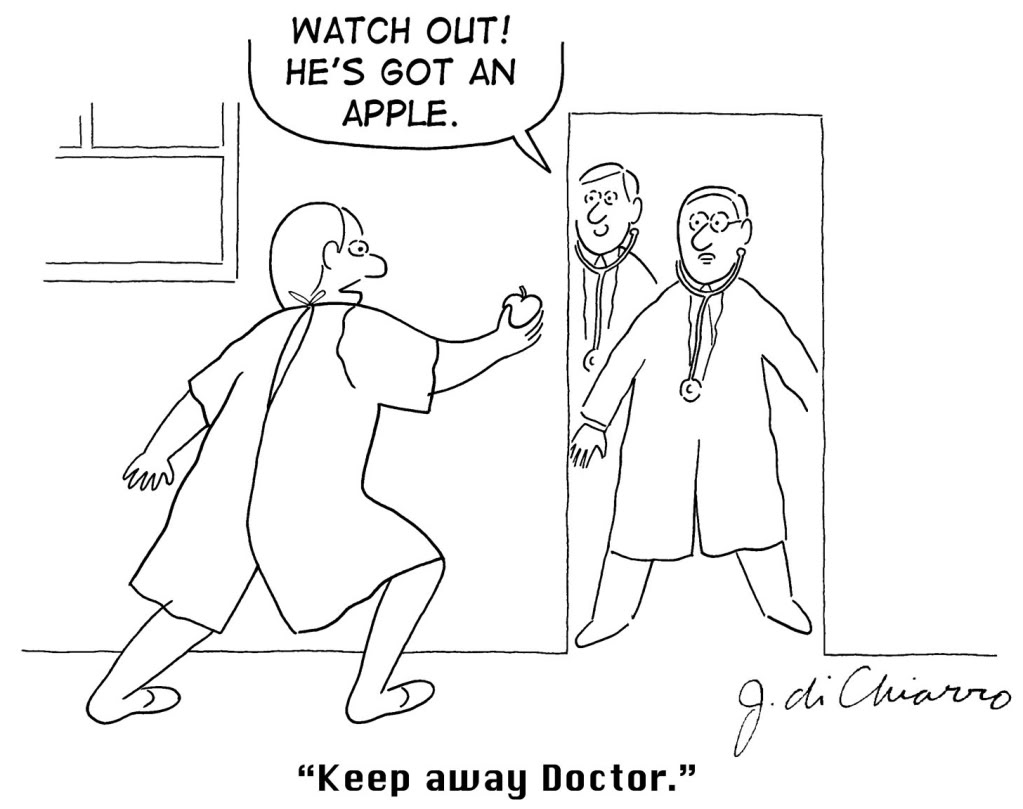
\includegraphics[scale=0.2]{apple-a-day.jpg}
		\pause

		An apple a day keeps the doctor away.

		Лучше предотвращать, чем отлаживать.
	\end{center}
\end{frame}

\begin{frame}{Причина}
	\begin{center}
		
\includegraphics[scale=0.2]{race-or-bug.jpg}
	\end{center}
	\begin{itemize}
		\item Многопоточные баги обычно тесно связаны с порядком выполнения операций.
		\item Операции выполняются в разном порядке каждый запуск, под отладчиком, в разном коде.
		\item Очень сложно ловить баг <<за руку>>.
		\item Корректная работа на куче тестов не означает отсутствие багов.
	\end{itemize}
\end{frame}

\begin{frame}{Как предотвращать}
	\begin{itemize}
		\item Явно расставляйте инварианты в комментариях: что чем защищено, в каком порядке захватывать мьютексы.
		\item Нарисуйте на бумажке все возможные состояния системы и проверьте, что инварианты выполняются.
		\item Минимизируйте количество мьютексов, если нет проблем со скоростью работы.
		\item Не используйте для синхронизации ничего, кроме мьютексов (в частности, явных \t{sleep} в программе быть не должно).
	\end{itemize}
\end{frame}

\begin{frame}{Как тестировать}
	\begin{itemize}
		\item Запускайте на больших тестах, в которых потоки работают медленно и часто происходит переключение.
		\item
			Если вы под 64-битным Linux (или Clang под Windows) "--- используйте thread sanitizer.
			Он хорош в нахождении некоторых гонок данных, \textit{происходящих во время выполнения}.
		\item
			Аналогично можно использовать Valgrind.
		\item
			На Windows можно поставить виртуальную машину с Linux и запускать там.
		\item
			Задавайте вопросы!
	\end{itemize}
\end{frame}


\end{document}
